\subsection{COUNTABILITY PROPERTIES OF SPACES OF CONTINUOUS FUNCTIONS}

THEOREM I. Let X be a compact space.

\begin{enumerate}
\def\labelenumi{\alph{enumi})}
\item
  If X is metrizable and if Y is any metrizable uniform space of countable type (Chapter IX, § 2, no. 8), then the metrizable space \(\mathcal{C}_{\mathbf{u}}(\mathbf{X};\mathbf{Y})\) of continuous mappings of X into Y, endowed with the topology of uniform convergence, is of countable type.
\item
  Conversely, if the metrizable space \(\mathcal{C}_{u}(\mathbf{X};\mathbf{R})\) is of countable type, then \(\mathbf{X}\) is metrizable.
\item
  Let \(d\) (resp. \(d'\) ) be a metric compatible with the topology of \(\mathbf{X}\) (resp. with the uniformity of \(\mathbf{Y}\) ); then \(\delta(f, g) = \sup_{x \in \mathbf{X}} d'(f(x), g(x))\) is a metric defining the uniformity of uniform convergence on the space \(\mathcal{C}(\mathbf{X}; \mathbf{Y})\) , the functions of \(\mathcal{C}(\mathbf{X}; \mathbf{Y})\) being bounded because \(\mathbf{X}\) is compact (no. 1). For each pair of integers \(m > 0\) , \(n > 0\) , let \(\mathbf{G}_{mn}\) be the set of functions \(f \in \mathcal{C}(\mathbf{X};\mathbf{Y})\) such that the relation \(d(x,x') \leqslant 1 / m\) implies \(d(f(x),f(x')) \leqslant 1 / n\) . Every function \(f \in \mathcal{C}(\mathbf{X};\mathbf{Y})\) is uniformly continuous (Chapter II, § 4, no. 1, Theorem 2) and therefore, for each \(n > 0\) , \(\mathcal{C}(\mathbf{X};\mathbf{Y})\) is the union of the sets \(\mathbf{G}_{mn}(m > 0)\) . Let \(\{a_1,\dots ,a_{p(m)}\}\) be a finite subset of \(\mathbf{X}\) such that the open balls with centres \(a_i\) and radii \(1 / m\) cover \(\mathbf{X}(1\leqslant i\leqslant p(m))\) ; and let \((b_r)_{r\in \mathbb{N}}\) be a countable sequence which is dense in \(\mathbf{Y}\) . For each mapping \(\varphi :[1,p(m)]\to \mathbf{N}\) , let \(\mathrm{H}_{\varphi}\) be the set of those \(f\in \mathbf{G}_{mn}\) such that \(d'(f(a_k),b_{\varphi (k)})\leqslant 1 / n\) for \(1\leqslant k\leqslant p(m)\) . By the definition of the \(b_r,\mathbf{G}_{mn}\) is the union of the sets \(\mathbf{H}_{\varphi}\) for \(\varphi \in \mathbf{N}^{p(m)}\) ; let \(\mathbf{C}_{mn}\) be the set of mappings \(\varphi \in \mathbf{N}^{p(m)}\) such that \(\mathrm{H}_{\varphi}\neq \emptyset\) , and for each \(\varphi \in \mathbf{C}_{mn}\) let \(g_{\varphi}\) be an element of \(\mathrm{H}_{\varphi}\) ; finally, let \(\mathrm{L}_{mn}\) denote the countable set of \(g_{\varphi}\) for \(\varphi \in \mathbf{C}_{mn}\) . Let \(f\in \mathbf{G}_{mn}\) , and let \(\varphi\) be an element of \(\mathbf{C}_{mn}\) such that \(f\in \mathrm{H}_{\varphi}\) ; then it follows immediately from the definitions that we have \(d'(f(x),g_{\varphi}(x))\leqslant 4 / n\) for all \(x\in X\) , i.e.~\(\delta (f,g_{\varphi})\leqslant 4 / n\) . Hence the union of the sets \(L_{mn}\) is dense in \(C_u(\mathbf{X};\mathbf{Y})\) , because for every integer \(n > 0\) and every \(f\in \mathcal{C}(\mathbf{X};\mathbf{Y})\) there exists \(m\) such that \(f\in G_{mn}\) , and we have just seen that the distance from \(f\) to \(L_{mn}\) is \(\leqslant 4 / n\) .
\item
  Let I = {[}0, 1{]}. Since \(\mathcal{C}_{u}(\mathbf{X};\mathbf{I})\) is a uniform subspace of \(\mathcal{C}_{u}(\mathbf{X};\mathbf{R})\) , it is of countable type. Let \((f_{n})\) be a sequence which is dense in \(\mathcal{C}_{u}(\mathbf{X};\mathbf{I})\) . Consider the product space \(K=I^{N}\) and the mapping \(\psi: x\to(f_{n}(x))\) of X into K, which is obviously continuous. The mapping \(\psi\) is injective; for, by definition of the sequence \((f_{n})\) , the relation \(f_{n}(x)=f_{n}(x')\) for all n implies, on passing to the limit, \(f(x)=f(x')\) for every function \(f\in\mathcal{C}(\mathbf{X};\mathbf{I})\) ; but this is impossible if \(x\neq x'\) by virtue of Axiom \((\mathrm{O}_{\mathrm{IV}})\) applied to the point x and to a neighbourhood V of x which does not contain \(x'\) (Chapter IX, §1, no. 5, Theorem 2). It follows that the compact space X is homeomorphic to the subspace \(\psi(\mathbf{X})\) of K (Chapter I, §9, no. 4, Theorem 2, Corollary 2); since K is metrizable and of countable type, so is \(\psi(\mathbf{X})\) and therefore so is X.
\end{enumerate}

Q.E.D.

COROLLARY. Let X be a locally compact space whose topology admits a countable base, and let Y be a metrizable uniform space of countable type.

\begin{enumerate}
\def\labelenumi{\alph{enumi})}
\item
  The space \(\mathfrak{L}\) of continuous mappings of \(\mathbf{X}\) into \(\mathbf{Y}\) which have a limit at infinity, endowed with the topology of uniform convergence in \(\mathbf{X}\) , is a metrizable space of countable type.
\item
  The space \(\mathcal{C}_{c}(\mathbf{X};\mathbf{Y})\) of continuous mappings of X into Y, endowed with the topology of compact convergence, is a metrizable space of countable type.
\item
  Let \(\mathbf{X}'\) be the compact space obtained by adjoining a point at infinity to \(\mathbf{X}\) (Chapter I, § 9, no. 8, Theorem 4); by definition, every function \(f \in \mathcal{L}\) can be uniquely extended to a continuous function \(\overline{f} \colon \mathbf{X}' \to \mathbf{Y}\) , and \(f \to \overline{f}\) is therefore a bijection of \(L\) onto \(\mathcal{C}(X'; Y)\) ; and this bijection is a homeomorphism of the space \(L\) onto \(\mathcal{C}_u(X'; Y)\) by Proposition 6 of §1, no. 6. Since \(X'\) is metrizable (Chapter IX, §2, no. 9, Proposition 16, Corollary) the result follows from Theorem 1, applied to \(X'\) and \(Y\) .
\item
  Let \((\mathbf{U}_{n})\) be a covering of X by relatively compact open sets, such that every compact subset of X is contained in some \(U_{n}\) (Chapter I, § 9, no. 9, Proposition 15, Corollary 1). If S is the set of the \(\overline{U}_{n}\) , the topology of compact convergence on C(X; Y) is the same as the topology of S-convergence. Consequently (§ 1, no. 2, Remark 3) the space \(\mathcal{C}_{c}(X; Y)\) is homeomorphic to a subspace of the product \(\prod_{n}\mathcal{C}_{u}(\overline{\mathbf{U}}_{n};\mathbf{Y})\) ; since each of the compact spaces \(\overline{U}_{n}\) has a countable base, it is metrizable (Chapter IX, § 2, no. 9, Proposition 16); each of the \(\mathcal{C}_{u}(\overline{\mathbf{U}}_{n};\mathbf{Y})\) is therefore metrizable and of countable type by Theorem 1, and hence so is \(\mathcal{C}_{c}(X;Y)\) .
\end{enumerate}

\pandocbounded{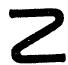
\includegraphics[keepaspectratio]{images/part002_29e6d4b6.jpg}}

Note that the space of all bounded continuous real-valued functions on R, endowed with the topology of uniform convergence, is not of countable type (Exercise 4).

